\graphicspath{{../loigiai/pic/}}

\begin{center}
	\textbf{ĐÁP ÁN CÁC BÀI TOÁN TRONG MỤC CHƠI CÙNG BI}
\end{center}
%\newpage
\begin{center}
	\textbf{ĐÁP ÁN BÀI TOÁN TRONG BÀI XẾP NAM CHÂM}
\end{center}
Bài 5\\
a.	Tương tự câu 2, bằng cách chia hình ra $4$ tầng ta đếm được số bi ở mỗi tầng là: $1,3,6,10$. Tổng số bi trong Hình 13 là
$$1+3+6+10= 20 \;(\text{viên}).$$
Hình 13 tạo bởi $10$ kim tự tháp mà mỗi cạnh là một thanh đen. Số thanh đen là: 
$$10\times 6=60 \;(\text{thanh}).$$


b.	Tương tự câu 4 ta lần lượt đếm được có $36$ tam  giác cạnh $1$, $20$ tam giác cạnh $2$, và $4$ tam giác cạnh $3$. Vâỵ tổng số tam giác có cạnh là các thanh đen là 
$$36+20+4=60  \;(\text{tam giác}).$$
\begin{center}
	\textbf{ĐÁP ÁN BÀI TOÁN TRONG BÀI TRIOMINO}
\end{center}
CÂU HỎI 17\\
Chúng ta thấy rằng để có “trận đồ” ở Hình 19, hai bạn Pi và Bi đã dùng hết các quân có đúng $2$ số $0$, và các quân có đúng hai số $1$. Ngoài ra, cho dù chơi tiếp thế nào sẽ không thể dùng quân gồm $3$ số $0$ và quân gồm $3$ số $1$ để chơi tiếp. Do vậy hai bạn không bao giờ có thể hết quân trên tay. “Trận đấu” này chắc chắn sẽ kết thúc với tình huống 2.
\newpage
%===============
\newpage
\begin{center}
	\textbf{ĐÁP ÁN CÁC BÀI TOÁN TRONG MỤC GIẢI TOẢN CÙNG BI}
\end{center}
\begin{center}
	\textbf{ĐÁP ÁN CÁC BÀI TOÁN TRONG BÀI ROBIN VÀ NHỮNG HÒN ĐẢO BÍ ẨN}
\end{center}
Đáp án câu $4$
\vskip 0.1cm
Để đếm được số chú ếch ở trên bờ và số chú ếch ở dưới ao, chúng ta cần phân biệt được hai miền: mặt ao và bờ ao. Do đó, số màu cần dùng để tô sẽ là một. Tiếp theo, do khóm sen nằm trên mặt ao nên để tô được mặt ao, ta cần đặt bút màu vào nơi có khóm sen trong Hình $1$, rồi tô màu sao cho trong quá trình tô, bút màu không rê qua đường viền đen ở bất cứ chỗ nào. Bằng cách đó, chúng ta sẽ thu được Hình $3$ dưới đây, mà ở đó, phần được tô màu chính là mặt ao. 
\begin{figure}[H]
	\centering
	\vspace*{-5pt}
	\captionsetup{labelformat= empty, justification=centering}
	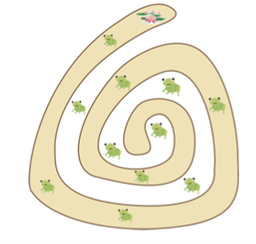
\includegraphics[width=0.4\linewidth]{1}
	\vspace*{-15pt}
\end{figure}
Bằng cách đếm trực tiếp, ta thấy, có sáu chú ếch ở miền không có màu và có năm chú ếch ở miền có màu.Vậy,ở trên bờ có sáu chú ếch và ở dưới ao có năm chú ếch. 
\vskip 0.1cm
Đáp án câu hỏi $5$:
\vskip 0.1cm
Để trả lời câu hỏi ta cần biết số kẹo mà mỗi người lấy được. Để biết bé lấy được mấy cái kẹo, chúng ta cần biết số kẹo màu đỏ chỉ nằm trong vòng dây màu cam; và để biết Bi lấy được mấy cái kẹo, chúng ta cần biết số kẹo màu xanh chỉ nằm trong vòng dây màu xanh lá cây. 
\vskip 0.1cm
Như thế, chúng ta cần phân biệt được ba miền: miền nằm trong vòng dây màu cam, miền nằm trong vòng dây màu xanh lá cây, và miền không nằm trong bất cứ vòng dây nào. Do đó, số màu cần dùng để tô sẽ là hai. Chúng ta sẽ dùng màu hồng để tô miền nằm trong vòng dây màu cam, và dùng màu cỏ úa để tô miền nằm trong vòng dây màu xanh lá cây. Khi đó, ta sẽ có hình dưới đây. 
\begin{figure}[H]
	\centering
	\vspace*{-5pt}
	\captionsetup{labelformat= empty, justification=centering}
	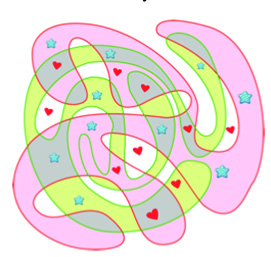
\includegraphics[width=0.4\linewidth]{2}
	\vspace*{-15pt}
\end{figure}
Bằng cách đếm trực tiếp, ta thấy bé sẽ lấy được hai chiếc kẹo (là những chiếc kẹo nằm ở nơi chỉ có màu hồng), còn Bi sẽ lấy được ba chiếc kẹo (là những chiếc kẹo nằm ở nơi chỉ có màu cỏ úa). Vậy, Bi lấy được nhiều kẹo hơn bé. Hi hi. 
\newpage
\begin{center}
	\textbf{ĐÁP ÁN CÁC BÀI TOÁN TRONG BÀI: BÀI TOÁN TRAO ĐỔI}
\end{center}
Bài toán 1: Cứ $2$ đùi thịt thú rừng đổi được $7$ sọt rau, quả nên $6$ đùi thịt thú rừng sẽ đổi được $3\times 7=21$ sọt rau, quả.%Cứ $2$ đùi thịt thú rừng đổi được $7$ sọt rau, quả nên $6$ đùi thịt thú rừng sẽ đổi được $3\times 7 =21$ sọt rau, quả. 

$21$ tấm da thú sẽ đổi được $14$ sọt rau quả nên $3$ tấm da thú sẽ đổi được $2$ sọt rau, quả. Như vậy với $9$ tấm da thú, bộ lạc sẽ đổi được $3\times 2= 6$ sọt rau, quả. %sọt rau, quả.

Tổng cộng bộ lạc đổi được số sọt rau, quả là: $$21+6=27 \;(\text{sọt}).$$

Bài toán 2\\
Do cứ mua $3$ bát to sẽ mua thêm $10$ bát nhỏ, người khách mua số bát nhỏ là:  $4\times 10= 40$ (cái).

Do cứ mua $5$ bát to sẽ mua thêm $2$ đĩa, người khách mua số đĩa là: $ 8\times 2= 16$ (cái).

Vì đã hết đĩa trong cửa hàng, chủ của hàng A cần đổi để được $16$ cái đĩa. Do $16$ chia $3$ được $5$ dư $1$, nên số bát to cần đem đi đổi không vượt quá $5$. Ta xét những trường hợp sau

-	$5$ bát to  =  $15$ đĩa, thiếu $1$ đĩa\\
-	$4$ bát to  =   $12$ đĩa, thiếu $4$ đĩa\\
-	$3$ bát to = $9$ đĩa, thiếu $7$ đĩa\\
-	$2$ bát to = $6$ đĩa, thiếu $10$ đĩa\\
-	$1$ bát to = $3$ đĩa, thiếu $13$ đĩa\\
-	$0$ bát to = $0$ đĩa, thiếu $16$ đĩa

Nhìn vào các trường hợp trên, ta thấy chủ của hàng A nên dùng 2 bát to và 6 bát nhỏ để đem đổi lấy 16 cái đĩa để bán cho khách hàng.

Bài toán 3.\\
Bác bán được $15$ trứng ngỗng nên số trứng vịt bán được là: 
$$5\times 7=35 \;\text{(quả)}.$$
Số trứng gà bán được là
$$5\times 5+ 7\times 2= 39 \;\text{(quả)}.$$
Số trứng chim cút bán được là:
$$7\times 10=70 \;\text{(quả)}.$$

Bài toán 4
Theo đề bài, giá bán 4 bông hồng sẽ bằng giá bán hai bông tulip. Vậy giá bán 1 bông hoa tulip cao gấp đôi giá bán một bông hoa hồng.

\textbf{Cuộc phiêu lưu của Mít Đặc và các bạn}
\vskip 0.1cm
$1.$ Đầu tiên, Nhanh Nhảu (đi $1$ phút) và Kèn Đồng (đi $2$ phút) cùng qua cầu -- mất đúng $2$ phút. Sau đó, Nhanh Nhảu quay lại mất $1$ phút cùng với chiếc đèn pin -- vậy là mất $3$ phút. Biết Tuốt (đi $5$ phút) và Mít Đặc (đi $10$ phút) cùng đi tiếp sang cầu -- vậy là mất tổng cộng $13$ phút. Bây giờ, Kèn Đồng sẽ qua lại mất 2 phút (và mất tổng cộng giờ là 15 phút) và đi sang cùng Nhanh Nhảu. Cuối cùng các chú tí hon sang hết bên kia cầu mất tổng cộng đúng 17 phút.
\vskip 0.1cm
2. Ta minh họa lại các thông tin của bài thơ của Mít Đặc qua hình sau.
\begin{figure}[H]
	\centering
	\vspace*{-5pt}
	\captionsetup{labelformat= empty, justification=centering}
	
\includegraphics[width=0.5\linewidth]{3}
	\vspace*{-15pt}
\end{figure}
Thay $3$
\includegraphics{4}  = 7
\includegraphics{5} từ phương trình thứ 2 vào phương trình thứ 1, ta được
\vskip 0.1cm
5
\includegraphics{6}  = 14
\includegraphics{5}  + 4
\includegraphics{5}  = 18
\includegraphics{5}.
\vskip 0.1cm
Như vậy, nếu Nước Đường có 10 quả cam và 6 quả táo thì Nước Đường sẽ có tổng cộng:
\vskip 0.1cm
10
\includegraphics{6}  + 6
\includegraphics{5}  = 36
\includegraphics{5}  + 6
\includegraphics{5}  = 42
\includegraphics{5}.
\vskip 0.1cm
Do 3
\includegraphics{4}  = 7
\includegraphics{5}  nên Nước Đường sẽ đổi được 18 quả lê.
\vskip 0.1cm
3.
\vskip 0.1cm
Đem cộng các chữ số của từng số trên nắp thùng ta được các số: 6, 4, 10, 2, 7, 9. Tổng của các số này là 29. Do số nước ngọt mà Mít Đặc mang tặng được chia làm 3 phần với số nguyên lít nên tổng số lít trong 5 thùng này là một số chia hết cho 3. Từ đó, thùng nước ngọt mà Mít Đặc giữ lại có thể tích là số chia cho 3 dư 2. Vậy thùng này chính là thùng có 20 lít nước ngọt.
\begin{figure}[H]
	\centering
	\vspace*{-5pt}
	\captionsetup{labelformat= empty, justification=centering}
	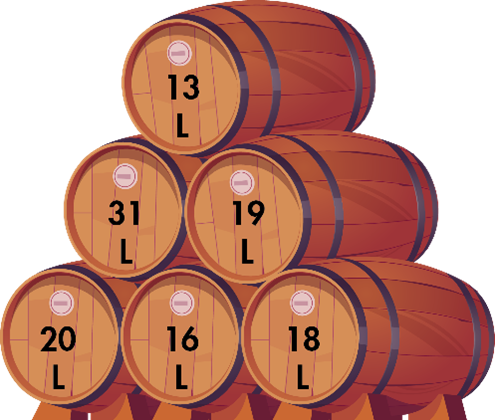
\includegraphics[width=0.3\linewidth]{7}
	\vspace*{-15pt}
\end{figure}
4. Để tiện lập luận, ta sẽ đánh số từ $1$ đến $16$ cho lưới ô vuông mà Thuốc Nước đưa cho Mít Đặc.
\begin{center}
	\def\myNotes{{{1,2,3,4},{5,6,7,8},{9,10,11,12},{13,14,15,16}}} 
	\begin{tikzpicture}[scale=0.7,color=cackithi]
		\foreach \x  in {1,2,...,4}
		\foreach \y in {1,2,...,4}
		{	
			\draw (\x,\y*-1) +(-.5,-.5) rectangle ++(.5,.5);
			\begin{scope}[shift={(\x,\y*-1)}]
				\pgfmathtruncatemacro{\r}{\myNotes[\y-1][\x-1]}
				\coordinate (C) at (0,0,0);
				\node (C) {$\color{black}\r$};
			\end{scope}
		}
	\end{tikzpicture}
\end{center}
Đầu tiên, Mít Đặc sẽ tô màu xanh trước. Do yêu cầu các ô cùng màu không nằm cùng hàng ngang, dọc hay chéo nên mỗi màu xanh sẽ nằm trên một hàng khác nhau. Nhận thấy màu xanh ở hàng $1$ không thể tô ở các ô góc. Thật vậy, nếu màu xanh đầu được tô ở ô góc số $1$ chẳng hạn, thì hàng thứ hai, ô màu xanh sẽ tô ở ô $7$ hoặc ô $8$.
\vskip 0.1cm
--	Nếu hàng $2$, màu xanh là ô $7$ thì hàng $3$ không có ô nào được tô mà thỏa mãn giả thiết. (Hình $1$)
\vskip 0.1cm
--	Nếu hàng $2$, màu xanh là ô $8$ thì hàng $3$ sẽ tô ở ô số $10$, nhưng hàng $4$ lại không có ô nào tô để thỏa mãn giả thiết. (Hình $2$)
\begin{center}
	\begin{tikzpicture}[scale=0.7]
		
		\fill[diendantoanhoc] (0,3) rectangle (1,4);
		\fill[diendantoanhoc] (2,2) rectangle (3,3);
		\draw (0.5,3.5) node {$\color{black}1$};
		\draw (2.5,2.5) node {$\color{black}7$};
		
		\draw[step=1.0,cackithi,thick] (0,0) grid (4,4);
	\end{tikzpicture}
	\quad
	\begin{tikzpicture}[scale=0.7]
		
		\fill[diendantoanhoc] (0,3) rectangle (1,4);
		\fill[diendantoanhoc] (1,1) rectangle (2,2);
		\fill[diendantoanhoc] (3,2) rectangle (4,3);
		\draw (0.5,3.5) node {$\color{black}1$};
		\draw (1.5,1.5) node {$\color{black}10$};
		\draw (3.5,2.5) node {$\color{black}8$};
		
		\draw[step=1.0,cackithi,thick] (0,0) grid (4,4);
	\end{tikzpicture}
	
	\textit{\color{toancuabi}Hình $1.$ \hspace*{60pt}  Hình $2.$}
\end{center}
Do đó, trên hàng đầu tiên, màu xanh chỉ có thể tô ở ô số $2$ hoặc số $3$.
\vskip 0.1cm 
Ta sẽ xét cho trường hợp tô ở ô số $2$, trường hợp ô số $3$ được thực hiện tương tự.
Khi màu xanh đầu được tô ở ô số $2$, thì hàng $2$ sẽ là ô số $8$, hàng $3$ là ô số $9$ và hàng $4$ là ô số $15$.  (Hình $3$)
\begin{center}
	\begin{tikzpicture}[scale=0.7]
		
		\fill[diendantoanhoc] (0,1) rectangle (1,2);
		\fill[diendantoanhoc] (2,0) rectangle (3,1);
		\fill[diendantoanhoc] (3,2) rectangle (4,3);
		\fill[diendantoanhoc] (1,3) rectangle (2,4);
		\draw (0.5,1.5) node {$\color{black}9$};
		\draw (2.5,0.5) node {$\color{black}15$};
		\draw (3.5,2.5) node {$\color{black}8$};
		\draw (1.5,3.5) node {$\color{black}2$};
		
		\draw[step=1.0,cackithi,thick] (0,0) grid (4,4);
	\end{tikzpicture}
	
	\textit{\color{toancuabi}\small Hình $3$.}
\end{center}
Tiếp đến, Mít Đặc tô $4$ màu còn lại. Do mỗi màu không thể cùng trên đường chéo, nên mỗi ô vuông ở mỗi góc tương ứng với một màu. Chẳng hạn, $4$ màu trên được tô trên $4$ góc như sau, các trường hợp khác được xét tương tự.
\begin{figure}[H]
	\centering
	\vspace*{-5pt}
	\captionsetup{labelformat= empty, justification=centering}
	\begin{tikzpicture}[scale=0.7]
		\fill[diendantoanhoc] (0,1) rectangle (1,2);
		\fill[diendantoanhoc] (2,0) rectangle (3,1);
		\fill[diendantoanhoc] (3,2) rectangle (4,3);
		\fill[diendantoanhoc] (1,3) rectangle (2,4);
		\fill[gocco] (0,0) rectangle (1,1);
		\fill[toanhocdoisong] (0,3) rectangle (1,4);
		\fill[yellow] (3,3) rectangle (4,4);
		\fill[lichsutoanhoc] (3,0) rectangle (4,1);
		
		\draw[step=1.0,cackithi,thick] (0,0) grid (4,4);
	\end{tikzpicture}
	\quad
	\begin{tikzpicture}[scale=0.7]
		\fill[diendantoanhoc] (0,1) rectangle (1,2);
		\fill[diendantoanhoc] (2,0) rectangle (3,1);
		\fill[diendantoanhoc] (3,2) rectangle (4,3);
		\fill[diendantoanhoc] (1,3) rectangle (2,4);
		\fill[gocco] (0,0) rectangle (1,1);
		\fill[toanhocdoisong] (2,2) rectangle (3,3);
		\fill[toanhocdoisong] (0,3) rectangle (1,4);
		\fill[toanhocdoisong] (1,0) rectangle (2,1);
		\fill[yellow] (3,3) rectangle (4,4);
		\fill[lichsutoanhoc] (3,0) rectangle (4,1);
		\draw (0.5,3.5) node {$\color{black}1$};
		\draw (2.5,2.5) node {$\color{black}7$};
		\draw (1.5,0.5) node {$\color{black}14$};
		
		\draw[step=1.0,cackithi,thick] (0,0) grid (4,4);
	\end{tikzpicture}
	\quad
	\begin{tikzpicture}[scale=0.7]
		\fill[diendantoanhoc] (0,1) rectangle (1,2);
		\fill[diendantoanhoc] (2,0) rectangle (3,1);
		\fill[diendantoanhoc] (3,2) rectangle (4,3);
		\fill[diendantoanhoc] (1,3) rectangle (2,4);
		\fill[gocco] (0,0) rectangle (1,1);
		\fill[toanhocdoisong] (1,0) rectangle (2,1);
		\fill[toanhocdoisong] (0,3) rectangle (1,4);
		\fill[toanhocdoisong] (3,1) rectangle (4,2);
		\fill[yellow] (3,3) rectangle (4,4);
		\fill[lichsutoanhoc] (3,0) rectangle (4,1);
		\draw (0.5,3.5) node {$\color{black}1$};
		\draw (3.5,1.5) node {$\color{black}12$};
		\draw (1.5,0.5) node {$\color{black}14$};
		
		\draw[step=1.0,cackithi,thick] (0,0) grid (4,4);
	\end{tikzpicture}
\caption{\small\textit{\color{toancuabi}Hình $4$ \hspace*{55pt} Hình $5$ \hspace*{55pt}Hình $6$}}
\end{figure}
Tiếp theo, bạn Mít Đặc chọn một màu và tô tiếp, chẳng hạn màu đỏ. Vị trí của $3$ ô màu đỏ có thể là $1$, $7$, $14$ hoặc $1$, $12$, $14$.Tuy nhiên, nếu màu đỏ tô ở các ô $1$, $12$, $14$ (Hình $6$) thì màu tím không có cách nào tô thỏa mãn. Do đó, màu đỏ sẽ được tô ở các ô: $1$, $7$, $14$. (Hình $5$)
\vskip 0.1cm
Từ đó, màu vàng sẽ được tô ở các ô: $4$, $5$, $11$, màu tím được tô ở các ô: $6$, $12$, $13$ và cuối cùng các ô còn lại là cho màu nâu: $3$, $10$, $16$. (Hình $7$)
\begin{center}
	\begin{tikzpicture}[scale=0.7]
		\fill[diendantoanhoc] (0,1) rectangle (1,2);
		\fill[diendantoanhoc] (2,0) rectangle (3,1);
		\fill[diendantoanhoc] (3,2) rectangle (4,3);
		\fill[diendantoanhoc] (1,3) rectangle (2,4);
		\fill[gocco] (1,2) rectangle (2,3);
		\fill[gocco] (3,1) rectangle (4,2);
		\fill[gocco] (0,0) rectangle (1,1);
		\fill[toanhocdoisong] (2,2) rectangle (3,3);
		\fill[toanhocdoisong] (0,3) rectangle (1,4);
		\fill[toanhocdoisong] (1,0) rectangle (2,1);
		\fill[yellow] (3,3) rectangle (4,4);
		\fill[yellow] (0,2) rectangle (1,3);
		\fill[yellow] (2,1) rectangle (3,2);
		\fill[lichsutoanhoc] (3,0) rectangle (4,1);
		\fill[lichsutoanhoc] (1,1) rectangle (2,2);
		\fill[lichsutoanhoc] (2,3) rectangle (3,4);
		
		\draw[step=1.0,cackithi,thick] (0,0) grid (4,4);
	\end{tikzpicture}
	
	\textit{\small\color{toancuabi}Hình $7.$}
\end{center}
Như vậy, bằng cách lập luận như trên, bạn Mít Đặc đã thực hiện được yêu cầu của họa sĩ Thuốc Nước rồi đấy. Hy vọng lần này bạn ấy sẽ vẽ được những bức chân dung đẹp hơn các bạn nhỉ.
\begin{figure}[H]
	\centering
	\vspace*{-5pt}
	\captionsetup{labelformat= empty, justification=centering}
	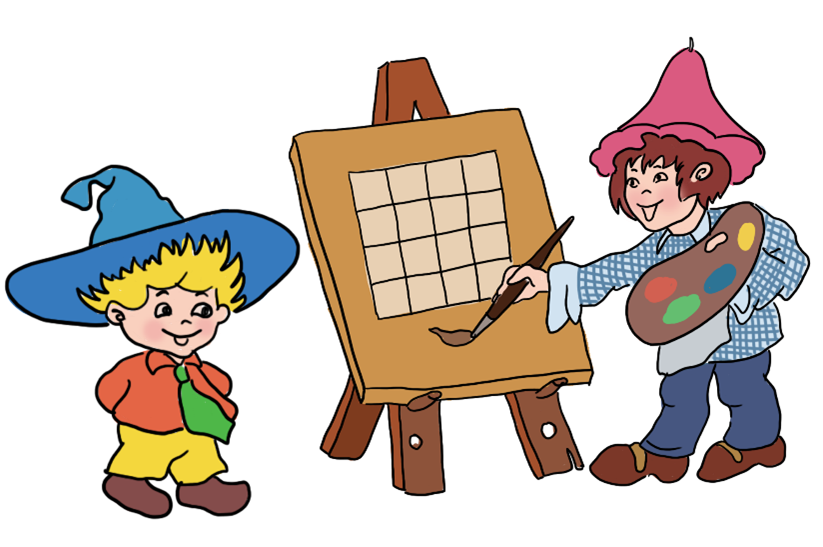
\includegraphics[width=0.5\linewidth]{8}
	\vspace*{-15pt}
\end{figure}
5. Nhận thấy quãng đường đi lên và đi xuống quả đồi của hai bạn là như nhau, mà vận tốc lúc xuống gấp 3 lần vận tốc lúc lên, nên thời gian lên dốc gấp 3 lần thời
gian xuống dốc. Tổng thời gian hai bạn đi lên và đi xuống quả đồi là 4 tiếng, vậy lúc lên các bạn đi mất 3 tiếng và lúc xuống các bạn đi mất 1 tiếng.
Như vậy, quả đồi dài 6km và quãng đường các bạn phải đi là 12km.
\vskip 0.1cm
6. Đổi: $1 \mbox{ giờ} = 60 \mbox{ phút}$ nên: 
\vskip 0.1cm
$\bullet$ $\dfrac{3}{4} \mbox{ giờ}$ = $\dfrac{3}{4}\times 60 \mbox{ phút}= \dfrac{3\times 60}{4}  \mbox{ phút}= \dfrac{180}{4}  \mbox{ phút}= 45 \mbox{ phút}.$ 
\vskip 0.1cm
$\bullet$ $1\dfrac{1}{2} \mbox{ giờ}= \dfrac{3}{2} \mbox{ giờ} = \dfrac{3}{2}\times 60  \mbox{ phút}= \dfrac{3\times 60}{2}  \mbox{ phút}= \dfrac{180}{2}  \mbox{ phút}= 90 \mbox{ phút}.$
\vskip 0.1cm
Tổng thời gian mà các chú tí hon tập luyện là:
\begin{align*}
	25 + 45 + 90= 160 \ (\textrm{phút}).
\end{align*}
Nếu các chú bắt đầu dạy lúc $7$ giờ $40$ phút thì sau $20$ phút sẽ là $8$ giờ. Vậy, khi 8 giờ thì còn phải luyện tập thêm
\begin{align*}
	160-20=140\ (\textrm{phút})
\end{align*}
nữa. Ta có 
\begin{align*}
	140= 2\times 60 +20
\end{align*}
nên $140$ phút $=2$ giờ và $20$ phút. Vậy, nếu các chú tí hon luyện tập $140$ phút kể từ lúc $8$ giờ thì các chú ấy sẽ kết thúc vào lúc  $10$ giờ $20$ phút.
\vskip 0.1cm
Đáp số: $10$ giờ $20$ phút.
\vskip 0.1cm
7.
\vskip 0.1cm
Tổng số phút các chú tí hon đã đi từ lúc bay qua đám mây là:
\vskip 0.1cm
40 + 60 + 10 + 80 + 20 = 210 (phút)
\vskip 0.1cm
Đổi 210 phút  = 3 giờ 30 phút.
\vskip 0.1cm
Thời gian các chú tí hon bay qua đám mây là: 11 giờ 30 phút. Do đó, các chú tí hon còn phải đi 2 tiếng mới đến được hòn đảo.
\vskip 0.1cm
8. 
\vskip 0.1cm
Lưu ý rằng một tuần dài gấp 7 lần so với một ngày. Điều này cho thấy kết quả của tính toán của Biết Tuốt không phải là 1 tuần cũng như không phải là 1 ngày. Tương tự, vì một tháng dài gấp 30, 31 hoặc 28, hay 29 lần so với một ngày và trong các câu trả lời của các chú tí hon không chứa số nào trong các số trên nên kết quả tính toán của Biết Tuốt không phải là một tháng. Như vậy, kết quả tính toán của Biết Tuốt phải hoặc là 1 giây, 1 phút hoặc là 1 giờ. Nếu kết quả tính toán là 1 giây hay 1 phút thì trong một giờ có 60 phút, trong một ngày có $60 \times 24 = 1440$ phút và trong một tuần có $1440\times 7 = 10080$ phút, do đó sai nhiều hơn 3600 lần so với tính toán! Như vậy, kết quả tính toán chỉ có thể là 1 giờ. Ta hãy kiểm tra lại điều này: - 1 giờ = 60 phút. - 1 phút = 60 giây. Vì thế, 1 giờ = $60\times 60 = 3600$ giây. - 1 ngày = 24 giờ. - 1 tuần = 7 ngày. Vì thế, 1 tuần = $7\times 24 = 168$ giờ. - 1 tháng có 30 ngày (như tháng 11) sẽ có số giờ là $30\times 24 = 720$ giờ. Như vậy, theo tính toán của Biết Tuốt thì kinh khí cầu sẽ tới thành phố mới sau 1 giờ.
\vskip 0.1cm
9. Ngôi nhà có số nhà là 3 được sơn màu vàng. Do ngôi nhà màu đỏ chỉ nằm cạnh đúng một ngôi nhà khác nên nó phải nằm ở một trong hai đầu của đoạn phố đó. Ngôi nhà màu xanh nằm cạnh ngôi nhà màu vàng và ngôi nhà màu đỏ. Thế nên thứ tự từ ngôi nhà màu đỏ tới đầu còn lại của con phố là đỏ, xanh, vàng. Như vậy, ngôi nhà màu vàng là ngôi nhà nằm chính giữa. Do đó, nhà của Đinh Ốc được sơn màu vàng.
\vskip 0.1cm
10. Do tổng số táo của bốn bạn là 100 và số táo của Bu Loong hái được gấp ba lần tổng số táo của ban bạn còn lại nên dễ thấy Bu Loong hai chuyển được 75 quả táo còn tổng số táo mà 3 bạn còn lại chuyển là 25. 
\begin{figure}[H]
	\centering
	\vspace*{-5pt}
	\captionsetup{labelformat= empty, justification=centering}
	
\includegraphics[width=1\linewidth]{9}
	\vspace*{-15pt}
\end{figure}
Do Mít Đặc chuyển được nhiều hơn 5 quả táo nên số táo mà cậu ấy chuyển được ít nhất là 6 quả.
\vskip 0.1cm
Nhận thấy nếu Mít Đặc chuyển được ít nhất là 7 quả thì số táo mà Mít Đặc chuyển ít nhất là 8 và số táo của Nhanh Nhảu ít nhất là 11. Khi đó, tổng số táo chuyển được của ba bạn ít nhất phải là 7 + 8 + 11 = 26 (mâu thuẫn).
\vskip 0.1cm
Vậy Mít Đặc chuyển được 6 quả táo. 
\vskip 0.1cm
+) Nếu Ngộ Nhỡ chuyển được 7 quả táo thì khi đó Nhanh Nhảu được 10 quả và tổng số táo của ba bạn là 23 khác 25. Vậy trường hợp này không xảy ra.
\vskip 0.1cm
+) Nếu Ngộ Nhỡ chuyển được 8 quả thì Nhanh Nhảu được 11 quả và ta được đẳng thức 6+8+11= 25.
\vskip 0.1cm
+) Nếu Ngộ Nhỡ chuyển trên 8 quả thì thấy ngay tổng số táo của ba bạn trên 25 quả và do vậy trường hợp này cũng không xảy ra.
\vskip 0.1cm
Vậy Mít Đặc chuyển được 6 quả táo, Ngộ Nhỡ chuyển được 8 quả, Nước Đường chuyển được 11 quả và Bu Loong nhờ “cơ khí hóa” chuyển được số táo nhiều nhất là 75 quả.
\vskip 0.1cm
11. 
Theo lời của các cô tí hon, lều của các cô còn có thể nhận số lượng khách là:
\begin{align*}
	18 : 2 = 9 (\text{người}).
\end{align*}
Mà lúc đó, lều đã chứa 3/ 4 số lượng khách so với khả năng của mình.
Như vậy, số khách mà lều còn có thể nhận so với khả năng của mình là:
\begin{align*}
	1- 3 /4 = 1/ 4 .
\end{align*}
Ta có sơ đồ về số lượng khách đã có và số lượng khách mà lều có thể nhận:
\begin{center}
	\begin{tikzpicture}[scale =0.6]
		\definecolor{upmaroon}{rgb}{0.48, 0.07, 0.07}
		\draw[very thick,color=red] (0,0)--(9,0);
		\draw[very thick, dash dot,color=green] (9,0)--(12,0);
		\draw[thick,color=black] (0, -0.1)--(0, 0.1) (3,-0.1)--(3,0.1) (6,-0.1)--(6,0.1) (9,-0.1)--(9,0.1) (12,-0.1)--(12,0.1);
		\node at (3,-0.8) {\textcolor{red}{Lượng khách}};
		\node at (3.2,-1.8) {\textcolor{red}{đã có}};
		\node at (9,-0.8) {\textcolor{green}{Lượng khách lều}};
		\node at (9,-1.8) {\textcolor{green}{có thể nhận}};
	\end{tikzpicture}
\end{center}
Như vậy, tổng số lượng khách mà lều có thể nhận là:
\begin{align*}
	9\times4 = 36 (\text{người}). 
\end{align*}
Ta có sơ đồ sau:
\begin{center}
	\begin{tikzpicture}[scale=0.6]
		\definecolor{upmaroon}{rgb}{0.48, 0.07, 0.07}
		\draw[very thick,color=blue] (0,0)--(8,0);
		\draw[very thick,color=orange] (8,0)--(12,0);
		\draw[thick,color=black] (0,-0.1)--(0,0.1) (4,-0.1)--(4,0.1) (8,-0.1)--(8,0.1) (12,-0.1)--(12, 0.1);
		\node at (4,-0.8) {\textcolor{blue}{Sức chứa của}};
		\node at (4.1,-1.8) {\textcolor{blue}{lều lớn}};
		\node at (10,-0.8) {\textcolor{orange}{Sức chứa của}};
		\node at (10,-1.8) {\textcolor{orange}{lều nhỏ}};
	\end{tikzpicture}
\end{center}
Từ đó suy ra số lượng khách mà lều nhỏ có thể chứa là: $36 : 3 = 12$ (người).
\vskip 0.1cm
12.
\vskip 0.1cm
Đinh Dép bắt đầu sơn từ điểm cách mép trái là 2 mét và kết thúc tại vị trí cách mép trái:
\begin{align*}
	2+9 = 11 (m).
\end{align*}
Ta biết rằng Lặng Lẽ kết thúc khi cách mép trái của hàng rào là 4 mét và thùng sơn của Lặng Lẽ sơn được 10 mét hàng rào. Vì thế nên Lặng Lẽ đã bắt đầu sơn từ vị trí cách mép trái của hàng rào là:
\begin{align*}
	4+10 = 14 (m).
\end{align*}
Như vậy, có tất cả 2 đoạn của hàng rào được sơn đúng một lớp sơn là:
\vskip 0.1cm
$1.$ đoạn hàng rào từ vị trí cách mép trái 2 mét cho tới vị trí cách mép trái 4 mét. Đây là đoạn hàng rào chỉ được sơn bởi Đinh Dép. Độ dài của đoạn này là
\begin{align*}
	4-2 = 2 (m).
\end{align*}
$2.$ đoạn hàng rào từ vị trí cách mép trái 11 mét cho tới vị trí cách mép trái 14 mét. Đây là đoạn hàng rào chỉ được sơn bởi Lặng Lẽ. Độ dài của đoạn này là:
\begin{align*}
	14-11 = 3 (m). 
\end{align*}
Như vậy, tổng độ dài của phần hàng rào được sơn bởi đúng một lớp sơn là:
\begin{align*}
	2+3 = 5 (m).
\end{align*}
\begin{center}
	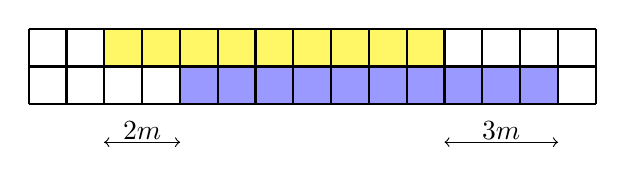
\begin{tikzpicture}[scale =0.48]
		\fill[blue!40!] (4,0) rectangle (14,1);
		\fill[yellow!60!] (2,2) rectangle (11,1);
		%\draw[thick,color=black] (2,1) grid (9,1);
		%\fill[blue] (2,1) rectangle (9,1);
		\draw[thick,color=black] (0,0) grid (15,2);
		%\fill[yellow] (4,0) rectangle (10,1);
		\draw [->] (4,-1)--(2,-1);
		\draw [->] (2,-1)--(4,-1);
		\node at (3,-0.7){$2m$}; 
		\draw [->] (11,-1)--(14,-1);
		\draw [->] (14,-1)--(11,-1);
		\node at (12.5,-0.7){$3m$}; 
	\end{tikzpicture}
\end{center}
13. Do bánh gato giá 13 đồng nên số bánh gato Bạch Tuyết mua sẽ ít hơn hay bằng 7. Do 1 đồng được hai xu kem nên số bánh xu kem là số chẵn. Khi đó có thể xảy ra các trường hợp sau
\begin{figure}[H]
	\centering
	\vspace*{-5pt}
	\captionsetup{labelformat= empty, justification=centering}
	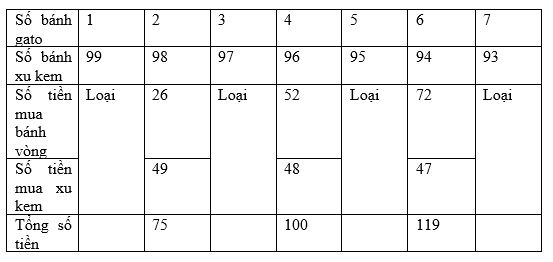
\includegraphics[width=1\linewidth]{10}
	\vspace*{-15pt}
\end{figure}
Vậy Bạch Tuyết có thể mua 4 cái bánh gato và 96 cái bánh xu kem.
\vskip 0.1cm
14.
Nếu Thuốc Viên không ra khỏi bệnh viện để đến nhà Mít Đặc sớm hơn 8 phút, thì trong trường hợp nếu cậu ta quay trở lại bệnh viện để lấy quần áo rồi tới nhà Mít Đặc, Thuốc Viên sẽ muộn không phải chỉ 10 phút mà tận 18 phút. Đó cũng là số thời gian cậu ta bị mất khi đi 2 lần quãng đường từ bệnh viện tới chỗ nhớ ra quên chưa thay quần áo bệnh viện. Vì vậy số thời gian cậu ta đi một lần từ bệnh viện tới chỗ sực nhớ là quên thay áo là 18∶2 = 9 phút, có nghĩa là cậu ta đã đi được 9/20 quãng đường.
\vskip 0.1cm
15.
Để thuận tiện trong việc đếm số quân, Mít Đặt có thể xếp các quân domino theo hàng, sao cho ô vuông đầu có số chấm vượt quá số chấm của ô vuông sau. Khi đó, toàn bộ quân domino của bộ mới có thể liệt kê theo bảng sau.
\begin{figure}[H]
	\centering
	\vspace*{-5pt}
	\captionsetup{labelformat= empty, justification=centering}
	
\includegraphics[width=0.9\linewidth]{11}
	\vspace*{-15pt}
\end{figure}
Ta thấy,
\vskip 0.1cm
-- Có 13 quân domino có ô vuông đầu là 0;
\vskip 0.1cm
-- Có 12 quân domino có ô vuông đầu là 1;
\vskip 0.1cm
-- Có 11 quân domino có ô vuông đầu là 2;
\vskip 0.1cm
-- $\ldots$
\vskip 0.1cm
Tiếp tục đếm như trên, cuối cùng có 1 quân domino có ô vuông đầu là 12.
\vskip 0.1cm
Như vậy, tổng số quân trong bộ domino mới là:
\begin{align*}
	13 + 12 + \ldots + 1 = \frac{14\times13}{2}=91.
\end{align*}
16.
Sau lần Nhanh Nhảu lấy 8 chiếc kẹo cuối cùng, trong hộp có đúng 8 chiếc, gấp đôi số kẹo sau lần trao đổi thứ hai. Vì vậy sau lần trao đổi kẹo thứ hai, trong hộp có 8:2=4 (chiếc kẹo). Trước khi Nhanh Nhau lấy mất 8 chiếc, số kẹo trong hộp phải là 4+8 = 12 (chiếc). Vậy sau lần
thứ nhất trong hộp có 12:2 = 6 chiếc. Trước khi Nhanh Nhảu xin 8 chiếc ở lần trao đổi thứ nhất, trong hộp có 6+8=14 (chiếc kẹo). Vậy ban đầu Mít Đặc có 14:2=7 (chiếc kẹo).
\vskip 0.1cm
Số kẹo cho và nhận giữa Mít Đặc và Nhanh Nhảu được tóm tắt trong bảng sau.
%Lần	Kẹo Mít Đặc trước khi được cho	Kẹo Mít Đặc sau khi được cho	Số kẹo Nhanh Nhảu lấy
%Lần 1	7	14	8
%Lần 2	6	12	8
%Lần 3	4	8	8
%Cuối cùng	0		
\begin{figure}[H]
	\centering
	\vspace*{-5pt}
	\captionsetup{labelformat= empty, justification=centering}
	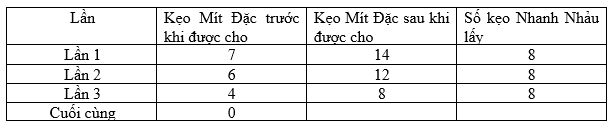
\includegraphics[width=1\linewidth]{12}
	\vspace*{-15pt}
\end{figure}
17. Gọi a là số thời gian tính theo phút từ lúc hai thi sĩ khởi hành tới lúc gặp nhau. Vận tốc của Kèn Đồng là g, vận tốc của Hoa Dại là d, khi đó ta có quãng đường từ nhà Hoa Dại tới điểm gặp là da, quãng đường từ nhà Kèn Đồng tới điểm gặp là ga. Sau khi gặp, Kèn Đồng đi tiếp 1.g còn Hoa Dại đi tiếp 4d.
\begin{figure}[H]
	\centering
	\vspace*{-5pt}
	\captionsetup{labelformat= empty, justification=centering}
	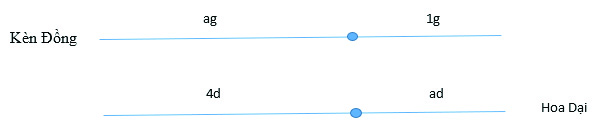
\includegraphics[width=1\linewidth]{13}
	\vspace*{-15pt}
\end{figure}
So sánh quãng đường từ lúc khởi hành đến lúc gặp theo hai cách, ta có 1g = da và 4d=ga.
\vskip 0.1cm
Nhân hai vế của hai đẳng thức trên với nhau ta có 4dg= a.a.gd. Giản ước cho gd ta có  a.a=4. Số a duy nhất thỏa mãn là a=2. Vậy Hoa Dại đi mất 2+4 = 6 phút, còn Kèn Đồng đi mất 2+1 = 3 phút.
\vskip 0.1cm
18. Gọi số cô tí hon là a, số túi mỗi cô đã may được là b. Khi đó, tổng số túi các cô tí hon đã làm được là ab. Mỗi cô tí hon đã tặng a túi cho mỗi chú tí hon, vì vậy có tất cả a×a số túi được tặng đi. Vì thế, cuối cùng các cô đã mang đến $ab - a\times a$ túi đến nhà Bạch Tuyết.
\vskip 0.1cm
Ta có $ab - a\times a =33$, hay là $a(b-a) = 33$. Do đó, a là ước số của 33. Theo đề bài, do $b - a > 1$ và $a>1$ nên a phải khác $1$ và $33$, vì thế $a=3$ hoặc $a= 11$.
\begin{figure}[H]
	\centering
	\vspace*{-5pt}
	\captionsetup{labelformat= empty, justification=centering}
	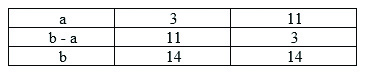
\includegraphics[width=1\linewidth]{14}
	\vspace*{-15pt}
\end{figure}
Trong cả hai trường hợp, chúng ta thấy số túi các cô tí hon may được đều bằng $14$.
\vskip 0.1cm
19.
Theo thông tin từ bài, người đầu tiên (người số 1) của Tròn Xoay phải là người số 14 của Mít Đặc. Vì thế người ở vị trí cuối cùng của Tròn Xoay sẽ là người số 13 theo cách đếm của Mít Đặc. Từ đó suy ra hiệu số của các số thứ tự của người số 94 và người cuối cùng theo cách đếm của Tròn Xoay cũng chính là hiệu số giữa số thứ tự của người số 7 và người số 13  theo cách đếm của Mít Đặc. Vì thế người cuối cùng là người số: $94+ 13-7=100$ theo cách đếm của Tròn Xoay.
\vskip 0.1cm
Vậy vòng tròn trong buổi vũ hội có 100 cô chú tí hon.
\begin{figure}[H]
	\centering
	\vspace*{-5pt}
	\captionsetup{labelformat= empty, justification=centering}
	
\includegraphics[width=0.5\linewidth]{15}
	\vspace*{-15pt}
\end{figure}
20. Theo hình vẽ bên, ta thấy số ngày dự tính làm kinh khí cầu bằng số chú tí hon tham gia vào làm nhân với mỗi ngày làm của mỗi chú.
Số chú tí hon tham gia vào làm kinh khí cầu là: $20 : 2 = 10$ (người)
\vskip 0.1cm
Số ngày cần thiết để làm kinh khí cầu là: $10 \times 4 = 40$ (ngày)
\begin{figure}[H]
	\centering
	\vspace*{-5pt}
	\captionsetup{labelformat= empty, justification=centering}
	
\includegraphics[width=0.5\linewidth]{16}
	\vspace*{-15pt}
\end{figure}
\newpage
\begin{center}
	{\color{red}{\textbf{ĐÁP ÁN PHẦN SUY LUẬN CÙNG BI}}}
\end{center}
\begin{center}
	\textbf{ĐÁP ÁN CÁC BÀI TOÁN TRONG BÀI SUMI VÀ NHỮNG CHIẾC MŨ SẮC MÀU}
\end{center}
Câu đố 4. % thực ra là câu 5

Jenny có thể trả lời ngay mình đội mũ màu gì chứng tỏ Sumi và Julia cùng đội mũ xanh. Sumi thấy bạn trả lời quả quyết như vậy thì chắc chắn mình đội mũ xanh rồi. Sumi nói đúng phải không các em?
\vskip 0.1cm
Câu đố 5. % thực ra là câu 4  , ở bài viết cần hoán đổi hai câu

Julia suy luận từ hai câu trả lời của hai anh chị Sumi và Jenny và trả lời bố là mình đội mũ màu đỏ. Thật vậy, Julia sẽ nghĩ như thế này: nếu mình đội mũ màu xanh và \\
1. nếu một trong hai anh chị đội mũ xanh chẳng hạn là anh Sumi thì lập tức chị Jenny sẽ biết là Jenny đội mũ đỏ vì chỉ có hai chiếc mũ xanh.\\
2.  nếu cả hai anh chị đội mũ đỏ. Khi đó, Sumi nhìn thấy một mũ xanh và một mũ đỏ sẽ không biết mình đội mũ gì. Jenny đã thấy Julia đội mũ xanh và biết Sumi không kết luận được mũ của chính mình nên Julia biết mũ của mình màu đỏ. Vậy Julia biết chính xác màu mũ của chị.

Nhưng cả hai anh chị không biết màu mũ của mình nên mũ của Julia phải là màu đỏ.

\newpage
\begin{center}
	\textbf{ĐÁP ÁN CÁC BÀI TOÁN TRONG BÀI SODUKO, PHẦN I VÀ II}
\end{center}
\begin{multicols}{2}
	\begin{figure}[H]
		\centering
		\vspace*{-5pt}
		\captionsetup{labelformat= empty, justification=centering}
		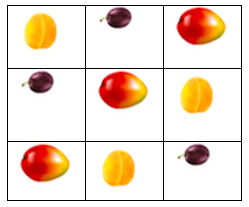
\includegraphics[width=0.9\linewidth]{sudoku1.png}
		\caption{\small{Bài 1}}
		\vspace*{-10pt}
	\end{figure}
	\begin{figure}[H]
		\centering
		\vspace*{-5pt}
		\captionsetup{labelformat= empty, justification=centering}
		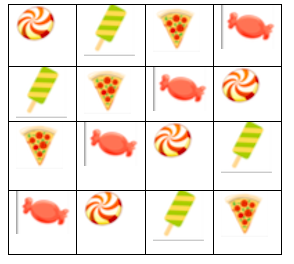
\includegraphics[width=0.9\linewidth]{sudoku2.png}
		\caption{\small{Bài 2}}
		\vspace*{-10pt}
	\end{figure}
	\begin{figure}[H]
		\centering
		\vspace*{-5pt}
		\captionsetup{labelformat= empty, justification=centering}
		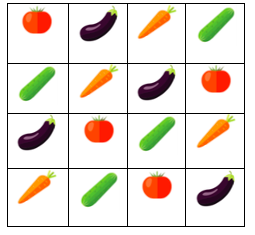
\includegraphics[width=0.9\linewidth]{sudoku3.png}
		\caption{\small{Bài 3}}
		\vspace*{-10pt}
	\end{figure}
	\begin{figure}[H]
		\centering
		\vspace*{-5pt}
		\captionsetup{labelformat= empty, justification=centering}
		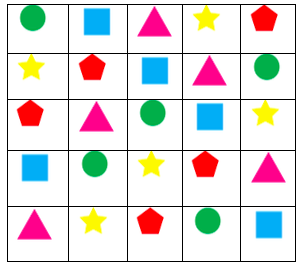
\includegraphics[width=0.9\linewidth]{sudoku4.png}
		\caption{\small{Bài 4}}
		\vspace*{-10pt}
	\end{figure}
	\begin{figure}[H]
		\centering
		\vspace*{-5pt}
		\captionsetup{labelformat= empty, justification=centering}
		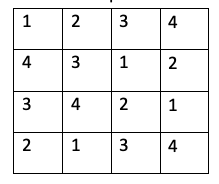
\includegraphics[width=0.9\linewidth]{sudoku5.png}
		\caption{\small{Bài 5}}
		\vspace*{-10pt}
	\end{figure}
	\begin{figure}[H]
		\centering
		\vspace*{-5pt}
		\captionsetup{labelformat= empty, justification=centering}
		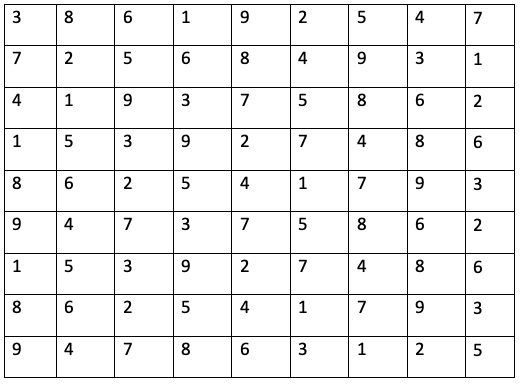
\includegraphics[width=0.9\linewidth]{sudoku6.png}
		\caption{\small{Bài 6}}
		\vspace*{-10pt}
	\end{figure}
\end{multicols}
\begin{center}
	\textbf{ĐÁP ÁN CÁC BÀI TOÁN TRONG BÀI PHỎNG VẤN THANH TRA LÊ KÍNH}
\end{center}
\textbf{Thổ ngữ châu Phi} 
\vskip 0.1cm
Trong ngôn ngữ địa phương, hai câu đầu tiên  ``KAF NAVCKI ROI" và "KIR ROI PALT" có chung từ ``ROI". Trong tiếng Việt, như thanh tra Lê Kính nói, các câu trên tương ứng với ``Lấy ba chiếc đi" và ``Hãy cất ba đồng xu" thì từ ``ba" là chung. Như vậy, nhiều khả năng là ``ROI" tương ứng với ``ba".
\vskip 0.1cm
Tương tự, nếu ta so sánh hai câu cuối ``KIR ROI PALT" và ``INOTI KAF KIR" thì ta nhận thấy chúng có chung từ ``KIR". Trong tiếng Việt, các câu này có nghĩa là ``Hãy cất ba đồng xu" và ``Lấy mấy đồng xu cẩn thận nhé" và chúng có chung từ ``đồng xu". Do đó, nhiều khả năng là ``KIR" có nghĩa là ``đồng xu". 
\vskip 0.1cm
Cũng như vậy, nếu ta so sánh câu đầu tiên và câu cuối cùng, ``KAF NAVCKI ROI" và ``INOTI KAF KIR", thì chúng có chung từ ``KAF".  Trong tiếng Việt, chúng có nghĩa là ``Lấy ba chiếc đi" và ``Lấy mấy đồng xu ra cẩn thận nhé", và có chung từ ``Lấy". Như vậy, từ ``KAF" có nghĩa là ``Lấy".
\vskip 0.1cm
Bây giờ, trong câu đầu tiên, ``KAF NAVCKI ROI" có nghĩa là ``Lấy ba chiếc đi" và ta biết ``KAF" nghĩa là ``Lấy" còn ``ROI" nghĩa là ``ba" nên ``NAVCKI" nghĩa là ``(mấy) chiếc bánh". Trong câu thứ hai, ``KIR ROI PALT" có nghĩa là ``Hãy cất ba đồng xu", ta biết ``KIR" nghĩa là ``đồng xu", ``ROI" nghĩa là ``ba" nên ``PAL" nghĩa là ``Hãy cất". Trong câu cuối cùng, ``INOTI KAF KIR" có nghĩa là ``Lấy mấy đồng xu ra cẩn thận nhé" ta biết rằng ``KAF" có nghĩa là ``Lấy", ``KIR" có nghĩa là ``đồng xu" nên ``INOTI" có nghĩa là ``cẩn thận (nhé)".
\vskip 0.1cm
Như vậy, để nói ``\textbf{Hãy cất mấy chiếc  bánh cẩn thận nhé}" ta chỉ cần nói ``\textbf{PAL NAVCKI INOTI}".

\vskip 0.1cm
\textcolor{timhieukhoahoc}{\textbf{ Du hành trên đại dương}}
\vskip 0.1cm
Các em hãy quan sát lá cờ Nhật Bản nhé. Lá cờ này không thể treo ngược được vì nó hoàn toàn đối xứng khi quay luật từ trên xuống dưới. Vậy Quản lý thiết bị $1$ đã nói dối và anh ta là kẻ trộm.
\vskip 0.1cm
\textbf{\color{quantoan} Thử thách sống còn}
\vskip 0.1cm
Việc Xuân Phong bị bịt mắt và giam vào phòng tối cho ta thấy anh ta không thể xác  định được viên thuốc nào màu đỏ và viên nào màu xanh. Nhưng bọn cướp cho anh ta chọn thuốc, có nghĩa là hai tay của Xuân Phong không bị trói. Và với hai tay được tự do như thế, Phong có thể chia đôi mỗi viên thuốc ra, cất riêng một nửa vào một nơi, và sau đó uống tất cả các nửa viên thuốc đã chia đôi mà không bị cất đi. Xuân Phong giờ có đúng $1$ viên đỏ và $1$ viên xanh để có đủ sức phá khóa và khống chế bọn cướp. Các em nhớ là cách này chỉ áp dụng được với các viên thuốc, không phải đối với viên nang (con nhộng) nhé. Và Xuân Phong là thám tử nên chắc cũng vô cùng khéo tay để bẻ đôi chính xác mỗi một viên ra để đảm bảo liều lượng.

\vskip 0.1cm
\textbf{\color{gocco}Chiếc mũ kỷ niệm} 
\vskip 0.1cm
Hai học trò đứng đầu hàng cùng đội mũ có cùng màu, đó là cách duy nhất mà tất cả ai cũng có thể đoán đúng.
\vskip 0.1cm
Thật vậy, ta gọi $3$ màu là A, B và C. Thám tử Xuân Phong xếp chiếc mũ theo thứ tự từ hàng dưới lên hàng trên là ABCC. Học trò ở cuối hàng nhìn thấy BCC. Và do đó cậu ta biết ngay mình đội mũ màu A, và nói to lên “A”.
\vskip 0.1cm
Học trò tiếp theo nhìn thấy CC và nghe học trò cuối hàng nói “A” nên cũng biết mình đội mũ màu B. Cậu ta trả lời ngay là “B”.
\vskip 0.1cm
Học trò thứ ba nghe câu trả lời của hai học trò vừa xong, biết họ đội các mũ khác màu nhau và nhìn thấy người đứng trước mình là C nên biết ngay mình đội chiếc mũ cùng màu C. Cậu ta sẽ trả lời được “C”.
\vskip 0.1cm
Học  trò đầu hàng giờ thì chả cần phải suy nghĩ gì nữa cũng biết được mình đội mũ C. Vậy là Xuân Phong đã trao được món quà động viên quý báu cho $4$ trò yêu của mình như vậy.
\vskip 0.1cm
\textbf{\color{toanhocdoisong}Ba chiếc hộp và cô thư ký}
\vskip 0.1cm
Lê Kính sẽ nhặt một bức thư trong hòm thư “Hòm thư chưa phân loại, lẫn cả thư gửi Xuân Phong và Lê Kính”. Nếu thư này đề người nhận là Xuân Phong, thì do cả $3$ hòm thư đều ghi sai nhãn, toàn bộ thư trong hòm đều gửi cho thám tử Phong. Vì thế nhãn đúng của hòm này là “Hòm thư riêng của Xuân Phong”.
\vskip 0.1cm
Vì thế hòm đã dán nhãn “Hòm thư riêng của Lê Kính” thực ra phải dán lại nhãn là “Hòm thư chưa phân loại, lẫn cả thư gửi Xuân Phong và Lê Kính”.
\vskip 0.1cm
Và do đó hòm thư đã được dán nhãn là “Hòm thư riêng của Xuân Phong” phải là “Hòm thư riêng của Lê Kính”.
\vskip 0.1cm

\textbf{\color{thachthuctoanhoc}Vị thám tử ẩn danh}
\vskip 0.1cm
Chúng ta sẽ phác thảo ra chiếc bàn vuông để dễ tưởng tượng và thử xác định nghề nghiệp của từng người thông qua $4$ thông tin trên nhé. 
\begin{center}
	\begin{tikzpicture}[scale=1.8,font=\small]
		\fill[color=cackithi!50] (0,1) rectangle (1,2);
		\draw[thin] (0,0) grid (1,3);
		\node at (0.5,2.5) {Bác sĩ};
		\node at (-0.5,1.5) {Mai};
		\draw[thin] (-1,1) grid (2,2);
	\end{tikzpicture}
\end{center}
Theo thông tin $2$:  Anh Trọng không thể ngồi bên tay phải cô Mai vì khi đó ngồi đối diện anh ta là Bác sỹ chứ không phải Thẩm phán. Vì vậy Trọng có thể ngồi ở đối diện  Mai hoặc ngồi bên tay trái cô ấy.
\vskip 0.1cm
Theo thông tin $3$: Cô Trang và anh Vinh ngồi cạnh nhau, vì vậy $2$ người còn lại là Mai và Trọng không thể ngồi đối diện. Vì vậy ta có cách xếp sau đây với anh Trọng.
\begin{center}
	\begin{tikzpicture}[scale=1.8,font=\small]
		\fill[color=cackithi!50] (0,1) rectangle (1,2);
		\draw[thin] (0,0) grid (1,3);
		\draw[thin] (-1,1) grid (2,2);
		\node at (0.5,2.7) {Bác sĩ};
		\node at (0.5,2.3) {Trọng};
		\node at (-0.5,1.5) {Mai};
		\node at (0.5,0.5) {Thẩm phán};
	\end{tikzpicture}
\end{center}
Thông tin $4$ có thể phát biểu lại là: phía bên tay phải một phụ nữ là một luật sư. Vì vậy, cùng với Thông tin $3$, ta xếp ngay được vị trí của anh Vinh và cô Trang ở $2$ chỗ còn lại như sau
\begin{center}
	\begin{tikzpicture}[scale=1.8,font=\small]
		\fill[color=cackithi!50] (0,1) rectangle (1,2);
		\draw[thin] (0,0) grid (1,3);
		\draw[thin] (-1,1) grid (2,2);
		\node at (0.5,2.7) {Bác sĩ};
		\node at (0.5,2.3) {Trọng};
		\node at (-0.5,1.5) {Mai};
		\node at (0.5,0.7) {Thẩm phán};
		\node at (0.5,0.3) {Trang};
		\node at (1.5,1.7) {Vinh};
		\node at (1.5,1.3) {Luật sư};
	\end{tikzpicture}
\end{center}
Và chúng ta giờ đều đã biết rõ cô Mai chính là vị Thám tử tư bí mật rồi, đúng không các em.

%=================

%=================
\newpage
\begin{center}
	\textbf{ĐÁP ÁN CÁC BÀI TOÁN TRONG MỤC TÌM HIỂU CÙNG BI}
\end{center}
%=================
\begin{center}
	\textbf{ĐÁP ÁN CÁC BÀI TOÁN TRONG BÀI HỌC LÀM THÁM TỬ}
\end{center}
Bài 1: Tay trái của Bi chỉ vào hướng Bắc, tay phải chỉ vào hướng Nam.

Bài 2: Ta xác định được hướng $12$ h như minh hoạ trong hình vẽ sau.
 \begin{figure}[H]
	\centering
	\vspace*{-5pt}
	\captionsetup{labelformat= empty, justification=centering}
	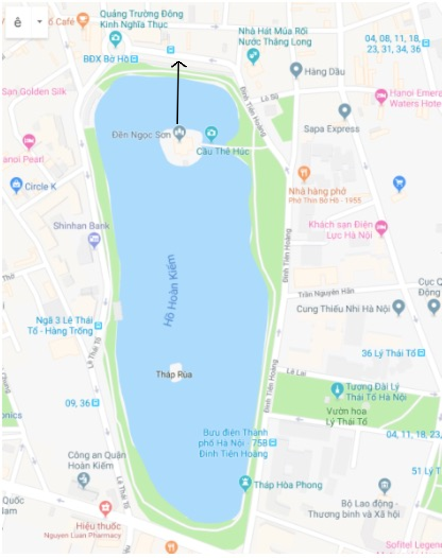
\includegraphics[width=0.5\linewidth]{bando.pdf}
	\vspace*{-15pt}
\end{figure}
 Như vậy ở hướng $11$ h ta có Quảng trường Đông Kinh Nghĩa Thục, hướng $1$ h là Nhà hát Múa rối Thăng Long. Còn Tháp Rùa ở hướng $6$ h.
%=================
\begin{center}
	\textbf{ĐÁP ÁN CÁC BÀI TOÁN TRONG BÀI ĐẾM HÌNH TAM GIÁC}
\end{center}
\textbf{Bài tập 1.}

Số tam giác trong Hình 4 là: $10$ tam giác.\\
Số tam giác trong Hình 5 là: $21$ tam giác.\\
\textbf{Bài tập 2.}

Số tam giác trong Hình 9 là: $40$ tam giác.\\
Số tam giác trong Hình 10 là: $31$ tam giác.\\
\textbf{Bài tập 3.}

Số tam giác trong Hình 15 là: $18$ tam giác.\\
Số tam giác trong Hình 16 là: $28$ tam giác.\\
Nhận xét. Số tam giác tạo bởi $n$ hình vuông dạng này là: $4\times 2\times n + 2\times (n-1)$.\\

\textbf{Bài tập 4.}

Số tam giác tạo thành từ tam giác có hoa văn kiểu tam giác có kích thước 6 là: $78$ tam giác.

\rule{1\textwidth}{0.1pt}
%=================
\begin{center}
	\textbf{ĐÁP ÁN ĐỐ VUI}
\end{center}

%Do_vui_Pi6_2021
$\pmb{1.}$
Mỗi ký hiệu đều có một đường thẳng đối xứng theo phương thẳng đứng. Nếu ta loại bỏ phần bên phải của mỗi ký hiệu đối với đường thẳng này thì phần còn lại của mỗi ký hiệu có hình dạng là một chữ số. Như vậy, biểu thức bên trên trở thành 2+6=8 và biểu thức bên dưới trở thành 1+3=? Vì thế câu trả lời phải là một ký hiệu mã hóa số 4. Đó chính là ký hiệu được cho bởi A).
\vskip 0.1cm
%Do_vui_Pi7_2019

$\pmb{2.}$ Đáp án c.
%Do_vui_Pi6_2019
\vskip 0.1cm
$\pmb{3.}$Đáp án là b).
\vskip 0.1cm
%Do_vui_Pi8_2019
$\pmb{4.}$ Các chữ số đã biết, lần lượt theo thứ tự là $1$, $4$, $1$, $5$, $9$, $2$, $6$, $5$. Đây là các chữ số sau dấu phảy của khai triển thập phân của số $\pi$ quên thuộc. Vì thế, số cần tìm chính là số $3$ vì

$$\pi = 3, 14159265\ldots$$
Như vậy, đáp án là c).
\vskip 0.1cm
%Do_vui_Pi9_2019
$\pmb{5.}$ Trả lời: mã số để mở khóa là 784.
\vskip 0.1cm
Ta có thể luận luận như sau. Theo b) thì chữ số  3  không xuất hiện trong mã. Như vậy, từ c) thì các chữ số  8 và 7 xuất hiện trong mã (nhưng nằm sai vị trí). Từ e) suy ra 6, 1 không xuất hiện trong mã. Từ a)  ta thấy 4 xuất hiện trong mã và nằm ở vị trí thứ 3. Từ đó, mã mở khóa phải là 784 hoặc 874. Trong hai khả năng này, dựa vào c), ta kết luận rằng mã mở khóa phải là 784 chứ không phải là 874.
\vskip 0.1cm

%Do_vui_Pi11_2019
$\pmb{6.}$ Câu trả lời đúng là B).
\vskip 0.1cm
%Do_vui_Pi4_2020
$\pmb{7.}$ Đáp án là B.


